\begin{figure}
    \centering
    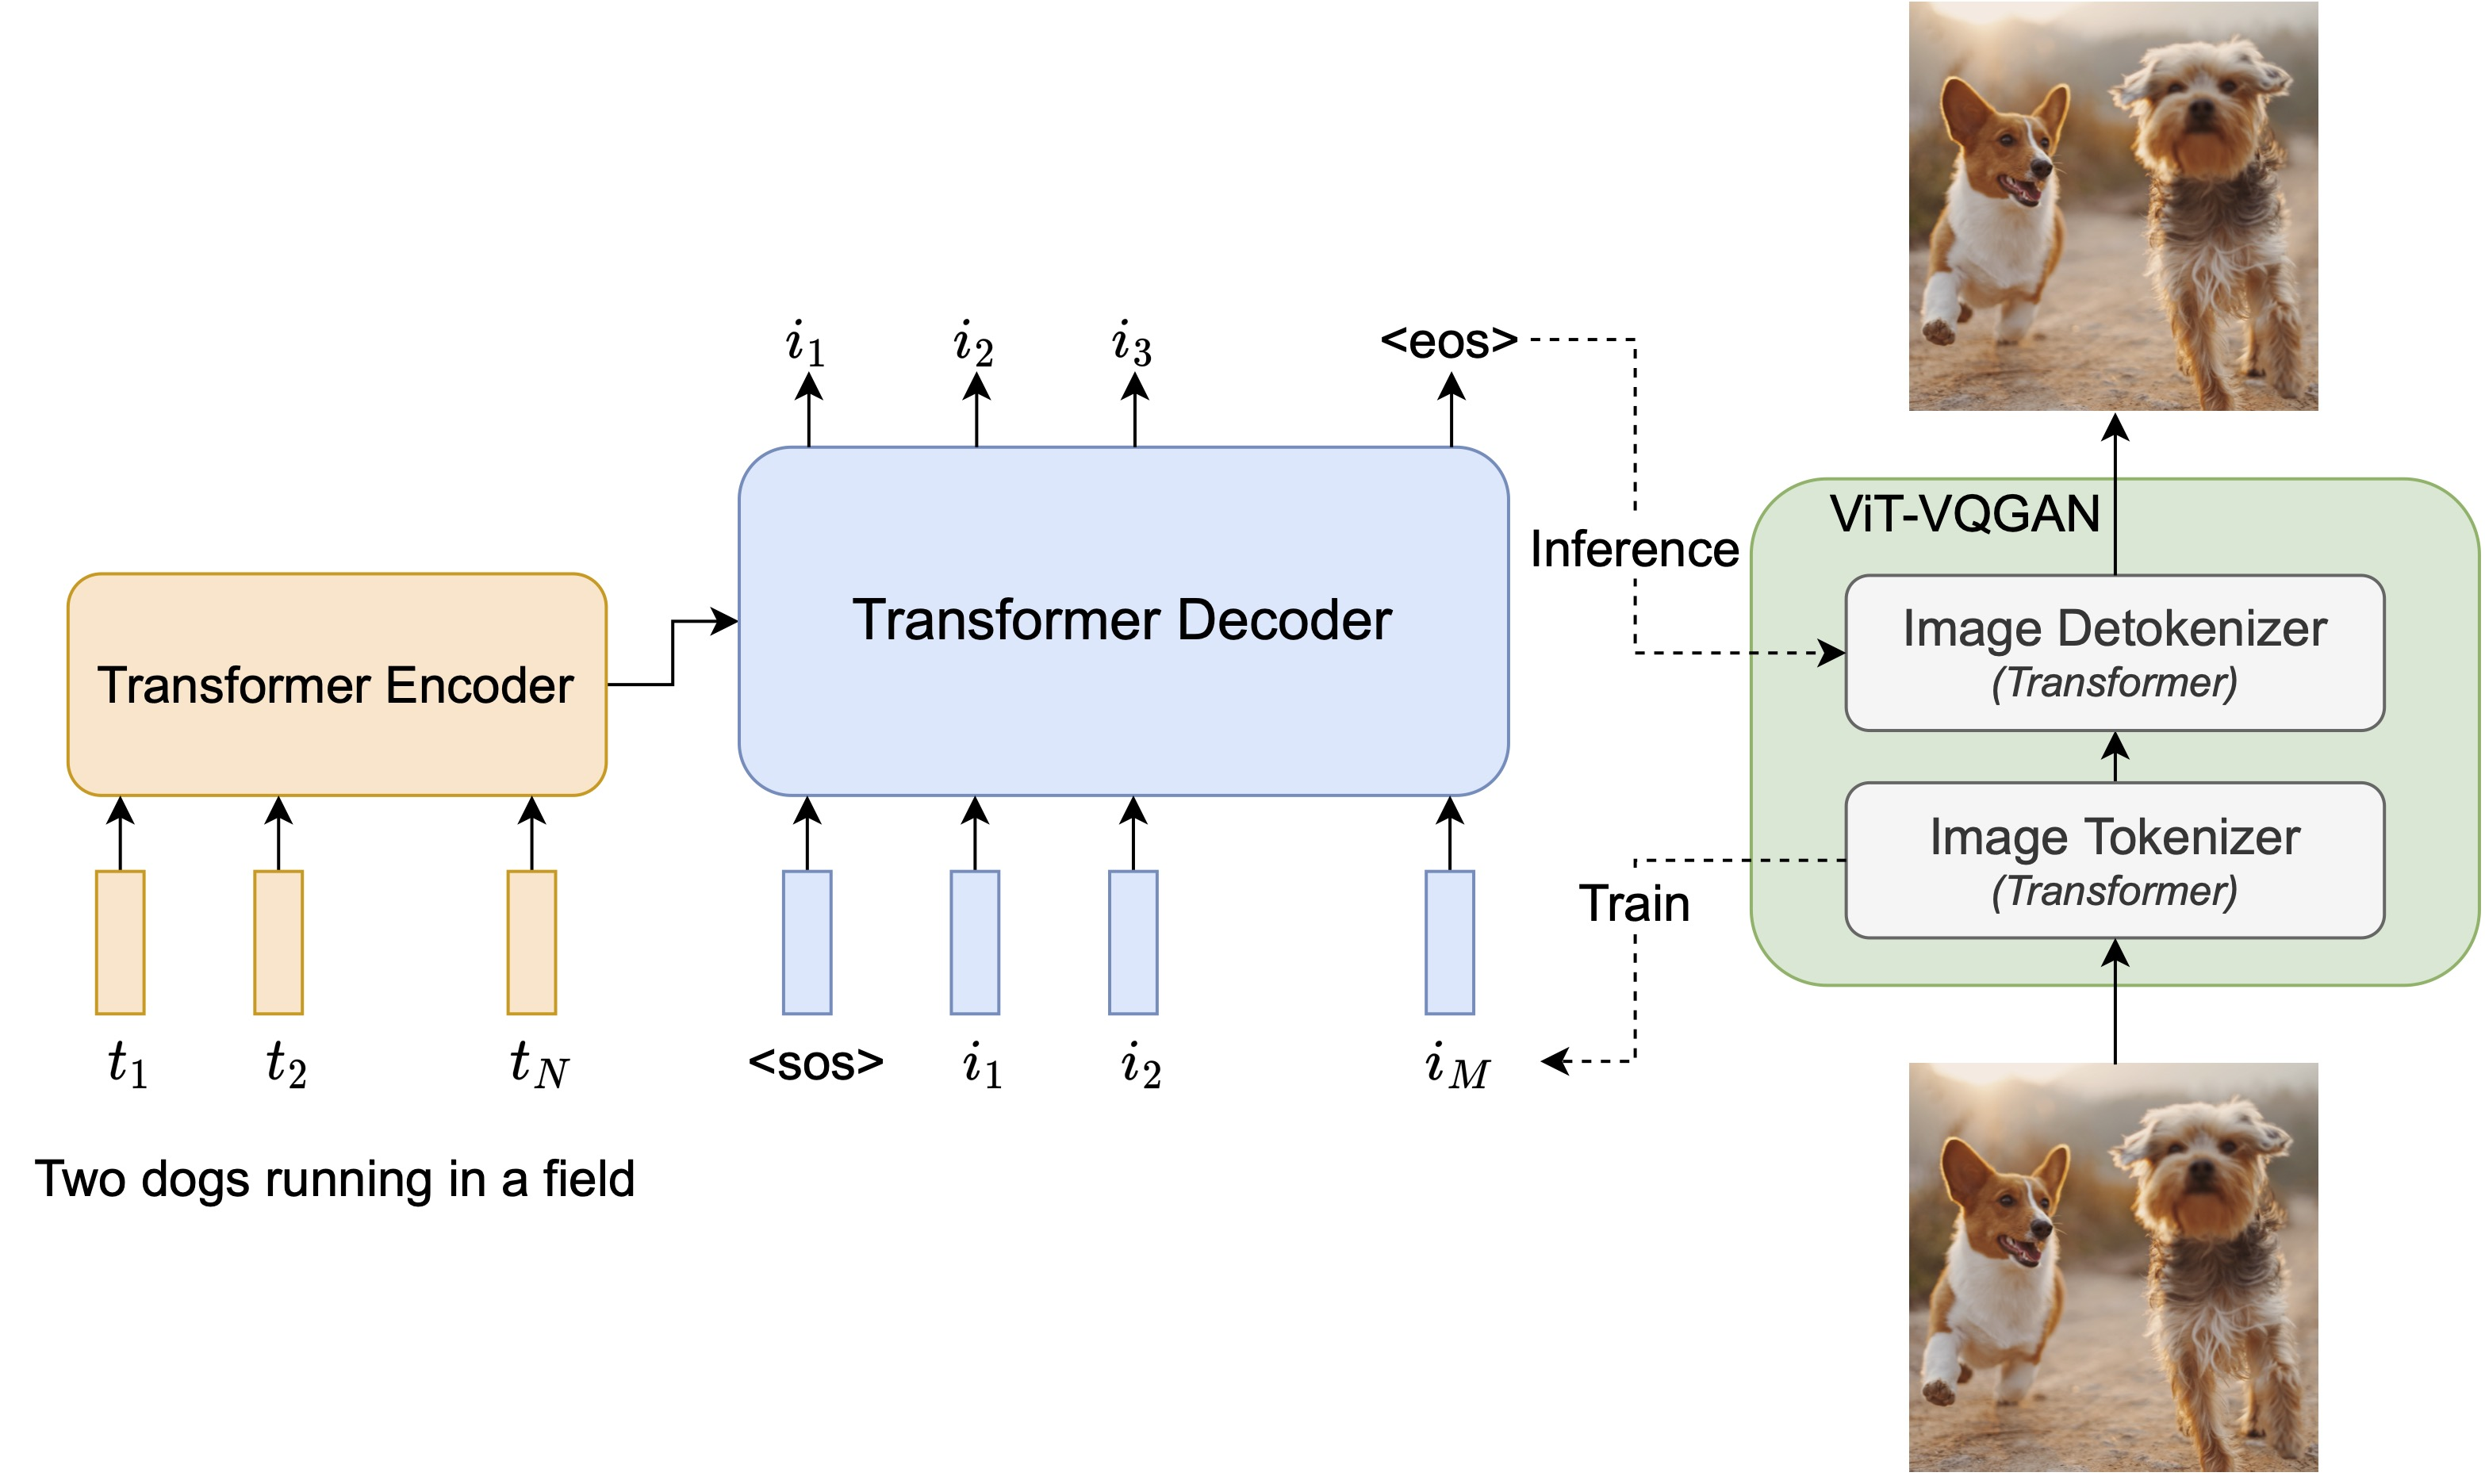
\includegraphics[width=0.75\textwidth]{figures/parti.jpg}
    \caption{Overview of \bdraw sequence-to-sequence autoregressive model (left) for text-to-image generation with ViT-VQGAN as the image tokenizer~\cite{yu2021vector} (right).}
    \label{figs:overview}
\end{figure}


\section{\bdraw Model}  
Similar to DALL-E~\cite{ramesh2021zero}, CogView~\cite{ding2021cogview}, and Make-A-Scene~\cite{gafni2022make}, \bdraw is a two-stage model, composed of an image tokenizer and an autoregressive model, as highlighted in Figure~\ref{figs:overview}. The first stage involves training a tokenizer that turns an image into a sequence of discrete visual tokens for training and reconstructs an image at inference time. The second stage trains an autoregressive sequence-to-sequence model that generates image tokens from text tokens. We describe details for these two stages below, together with other techniques for building high-performing autoregressive text-to-image models, such as text encoder pretraining, classifier-free guidance, and reranking.


\subsection{Image Tokenizer} \label{secs:tokenizer}
Autoregressive text-to-image models must linearize 2D images into 1D sequences of patch representations. In the limit, these are just pixels, as with iGPT~\cite{chen2020generative}, but this requires modeling very long sequences even for small images (\eg, a \(256{\times256}\times3\) RGB image leads to 196,608 rasterized values). Worse, it is based on a very low-level representation of the inputs rather than a richer one informed by the position of a pixel in the context of the image. Previous work~\cite{van2017neural, ramesh2021zero, yu2021vector, gafni2022make} addressed this problem by using a discrete variational auto-encoder to learn quantized representations of image patches over a collection of raw images. Instead of learning representations that can take any value in the latent space, a visual codebook is learned that maps a patch embedding to its nearest codebook entry, which is a learned and indexable location in the latent space. These entries can be thought of as visual word \textit{types}, and the appearance of any of these words in a patch in a given image is thus an image \textit{token}.

To be most useful for the second stage model, the image tokenizer needs to learn an effective visual codebook that supports balanced usage of its entries across a broad range of images. It also must support reconstruction of a sequence of visual tokens as a high-quality output image. We use ViT-VQGAN \cite{yu2021vector} with techniques including \(\ell_2\)-normalization codes and factorized codes, which contribute to training stability, reconstruction quality and codebook usage. A ViT-VQGAN image tokenizer is trained with the same losses and hyper-parameters as~\cite{yu2021vector} on images of our training data (see Section~\ref{secs:data}). We first train a ViT-VQGAN-Small configuration (8 blocks, 8 heads, model dimension 512, and hidden dimension 2048 as shown in Table 2 of~\cite{yu2021vector}, with about 30M total parameters), and learn 8192 image token classes for the codebook. We note that the second stage autoregressive encoder-decoder \textit{training} only relies on the encoder and the codebook of a learned image tokenizer. To further improve visual acuity of the reconstructed images after second-stage encoder-decoder training, we freeze the tokenizer's encoder and codebook, and finetune a larger-size tokenizer decoder (32 blocks, 16 heads, model dimension 1280, and hidden dimension 5120, with about 600M total parameters). We use \(256{\times}256\) resolution for the image tokenizer's input and output.

We notice visual pixelation patterns in some of the output images of ViT-VQGAN when zooming in (see Appendix~\ref{secs:appendix_pixelation}), and further find ill-conditioned weight matrices of the output projection layer before the sigmoid activation function. As a fix, we remove the final sigmoid activation layer and the logit-laplace loss, exposing the raw values as RGB pixel values (in range [0, 1]). Conveniently, this fix can be hot-swappable into an already trained image tokenizer by finetuning the decoder.

Finally, while images of resolution \(256{\times256}\) capture most of the contents, structures and textures, higher-resolution images have greater visual impact. To this end, we employ a simple super-resolution module on top of the image tokenizer, shown in Figure~\ref{figs:super_resolution}. Stacked convolutional layers with residual connections are used as the super-resolution network module following WDSR~\cite{yu2018wide} (12 residual blocks with 128 channels). It is learned with the same losses of ViT-VQGAN (perceptual loss, StyleGAN loss and \(\ell_2\) loss with same loss weighting in~\cite{yu2021vector}), mapping from reconstructed images to higher-resolution reconstructed images. The super-resolution module has about 15M parameters for the \(512{\times}512\) version and about 30M parameters for the \(1024{\times}1024\) version. We note that diffusion models could also be used here as iterative refinement super-resolution modules, as also demonstrated in DALL-E 2~\cite{ramesh2022hierarchical} and Imagen~\cite{imagen}, either with or without conditioning on text inputs.


\begin{figure}[t]
    \centering
    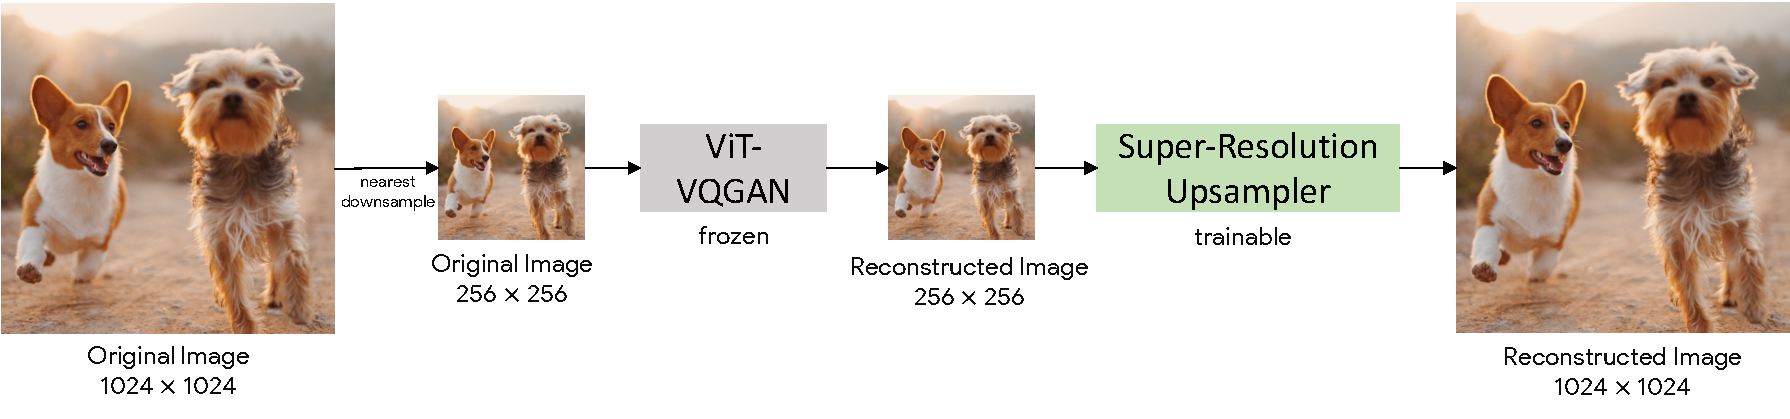
\includegraphics[width=\textwidth]{figures/sr_vit_vqgan.pdf}
    \caption{A learned super-resolution module to upsample \(256\times256\) images to higher-resolution \(1024\times1024\) ones based on a frozen ViT-VQGAN image tokenizer. The super-resolution module takes \(256\times256\) images as inputs without conditioning on text inputs.}
    \label{figs:super_resolution}
\end{figure}

\subsection{Encoder-Decoder for Text-to-Image Generation}
\begin{table}[t]
\centering
\resizebox{1.0\textwidth}{!}{%
\begin{tabular}{@{}lccccccc@{}}
    \toprule
    \textbf{Model} & \textbf{Encoder Layers} & \textbf{Decoder Layers} & \textbf{Model Dims} & \textbf{MLP Dims} & \textbf{Heads} & \textbf{Total Params}\\ 
    \midrule
    \bdraw-350M & 12 & 12 & 1024 & \pz4096 & 16 & 350M \\
    \bdraw-750M & 12 & 36 & 1024 & \pz4096 & 16 & 750M \\
    \bdraw-3B & 12 & 36 & 2048 & \pz8192 & 32 & \pzz3B \\
    \bdraw & 16 & 64 & 4096 & 16384 & 64 & \pz20B \\
    \bottomrule
\end{tabular}
}\\[.3cm]
\caption{\label{tabs:bdraw_variants} Size variants of \bdraw. Both encoder and decoder are based on Transformers~\cite{vaswani2017attention}. The self-attention layer in decoder transformer is causally masked. Parameters of ViT-VQGAN image tokenization are not included in the total parameter count and can be found in Section~\ref{secs:tokenizer}.}
\end{table}

As shown in Figure~\ref{figs:overview}, a standard encoder-decoder Transformer model is trained at the second stage, by treating text-to-image as a sequence-to-sequence modeling problem. The model takes text as input and is trained using next-token prediction of rasterized image latent codes generated from the first stage image tokenizer. For text encoding, we build a sentence-piece model~\cite{sennrich2015neural, kudo2018sentencepiece} of vocabulary size 16,000 on a sampled text corpus from the training data (Section~\ref{secs:data}). Image tokens are produced by a learned ViT-VQGAN image tokenizer (see Section~\ref{secs:tokenizer}). At inference time, the model samples image tokens autoregressively, which are later decoded into pixels using the ViT-VQGAN decoder.

We use a maximum length of text tokens of 128, and the length of image tokens are fixed to 1024 (\ie, \(32{\times}32\) latent codes from a \(256\times256\) input image). As an example, the 67-word description of the Starry Night prompt given in Figure~\ref{figs:teaser} has a total length of 92 text tokens. All models use conv-shaped masked sparse attention~\cite{child2019generating}. We train four size variants ranging from 350 million to 20 billion parameters, as detailed in Table~\ref{tabs:bdraw_variants}. Specifically, we configure the Transformers following previous practice of those in scaling language models with default expansion ratio of \(4\times\) in MLP dimensions. We double the number of heads when the model dimension is doubled. In the current scaling variants, our configuration prefers a larger decoder for modeling image tokens and as a result the decoder has more layers (\eg, \(3\times\) in the 3B model and \(4\times\) in the 20B model).

Most of the existing two-stage text-to-image generation models, including DALL-E~\cite{ramesh2021zero}, CogView~\cite{ding2021cogview} and Make-A-Scene~\cite{gafni2022make}, are decoder-only models. We found that at the model scale of 350-million to 750-million parameters, the encoder-decoder variants of \bdraw outperformed decoder-only ones, both in terms of training loss and text-to-image generation quality in our early exploration. We thus chose to focus on scaling the encoder-decoder models.

\subsection{Text Encoder Pretraining}
The encoder-decoder architecture also decouples text encoding from image-token generation, so it is straightforward to explore warm-starting the model with a pretrained text encoder. Intuitively, a text encoder with representations based on generic language training should be more capable at handling visually-grounded prompts. We pretrain the text encoder on two datasets: the Colossal Clean Crawled Corpus (C4)~\cite{raffel2019exploring} with BERT~\cite{devlin2018bert} pretraining objective, and our image-text data (see Section \ref{secs:data}) with a contrastive learning objective (image encoder from the contrastive pretraining is not used). After pretraining, we continue training both encoder and decoder for text-to-image generation with softmax cross-entropy loss on a vocabulary of 8192 discrete image tokens.

The text encoder after pretraining performs comparably to BERT \cite{devlin2018bert} on GLUE (see Appendix~\ref{secs:appendix_encoder_pretraining}, Table~\ref{table:glue_results}); however, the text encoder degrades after the full encoder-decoder training process on text-to-image generation. We leave this observation as a future research topic on the difference and unification of generic language representation and visually-grounded language representation. Still, the text-encoder pretraining \textit{marginally} helps text-to-image generation loss with 3B-parameter \bdraw models, so pretraining is used by default in our 20B model. We provide detailed training loss, GLUE evaluation of text encoders, and some qualitative comparison in Appendix~\ref{secs:appendix_encoder_pretraining}.

\subsection{Classifier-Free Guidance and Reranking} \label{secs:sampling_cf_coca}
Classifier-free guidance~\cite{ho2021classifier} (CF-guidance in short) is critical in the context of improving the sample quality of diffusion models~\cite{nichol2021glide, ramesh2022hierarchical, imagen} without pretrained classifiers. In this setup, a generative model $G$ is trained to be able to perform unconditional generation $G(\mathbf {z})$ (where $\mathbf {z}$ represents random noise) and conditional generation $G(\mathbf {z}, \mathbf{c})$ (where $\mathbf{c}$ represents some condition, such as language descriptions). It is implemented as randomly dropping out the conditional vector (masking out or switching to a learned embedding) with some probability. During the inference process, sampling of an output $I$ is done by using a linear combination of the unconditional and conditional predictions:
\begin{equation}  \label{eq:cf_eq}
I = G(\mathbf {z}) + \lambda (G(\mathbf {z}, \mathbf{c}) - G(\mathbf {z})),
\end{equation}
where $\lambda$ is a hyperparameter representing the weight of classifier-free guidance. Intuitively, it decreases the unconditional likelihood of the sample while increasing the conditional likelihood, which can be viewed as encouraging alignment between the generated sample and the text condition.

Classifier-free guidance has been similarly applied in the context of autoregressive models for text-to-image generation~\cite{crowson2021classifier, gafni2022make} to great effect. Make-A-Scene~\cite{gafni2022make} finetunes the model by randomly replacing the text prompts with padded tokens. During inference, tokens are sampled from a linear combination of logits sampled from an unconditional model and a conditional model on a text prompt. We also apply CF-guidance in \bdraw, and find it has a significant improvement on the output image-text alignment, especially on challenging text prompts.

With batch-sampled images per text prompt, contrastive reranking is used in DALL-E~\cite{ramesh2021zero} which produces image-text alignment scores after the generation. We apply contrastive reranking in our work and find it is complementary to classifier-free guidance. Compared with the 512 images used in DALL-E~\cite{ramesh2021zero}, we sample just 16 images per text prompt for the experiments reported in this paper. We rerank each output set based on the alignment score of image and text embedding of a Contrastive Captioners model (CoCa)~\cite{yu2022coca}. A CoCa base-size model (Table 1 in~\cite{yu2022coca}) is trained on the same dataset with details in Section~\ref{secs:data}. We note that reranking over a small set of batch-sampled images is computationally cheap in the text-to-image sampling process, and produces helpful image-text alignment scores among diverse image outputs.